%!TEX root = ../main.tex
%%%%%%%%%%%%%%%%%%%%%%%%%%%%%%%%%%
% Links:
%
% Difficulty:
% Companies: 
%%%%%%%%%%%%%%%%%%%%%%%%%%%%%%%%%%

\chapter{Verify BST property}
\label{ch:verify_BST}
\section*{Introduction}
Data structures is a topic that lies at the heart of the entire field of computer science and of virtually every computer code running around the globe.
Algorithms are built around particular data arrangements and there are some arrangements that are more convenient than others 
and often choosing the right one could mean the difference between waiting years for a particular algorithm to come to completion versus seconds. 

Among the vast number of the mainstream data structures, trees, and especially the binary kind, are probably one of the most used because they naturally allow representing hierarchical data which is ubiquitous and at the basis, DOM \footnote{Document Object Model is a way of representing documents as trees wherein each node is an object represents a part of the document (See Figure \ref{fig:verify:DOM}).} (XML,HTML) and  JSON documents, which lies at the heart of the Wolrd Wide Web.
Trees are also fundamental for compilers as they are used to represent the syntactic structure of a source code for programming languages.

Trees can be defined recursively as a collection of nodes, which contains some data and a lsit of references to other nodes, the "children". There is a special node called the root with the property that no other nodes have reference to it. Moreover, a node can only be referenced once (i.e. it can have one and only one father). See Figure \ref{fig:verify:generic_tree} for an example of a generic tree.



\begin{figure}
	\vspace*{-0.5in}
	\centering
	\begin{subfigure}[t]{0.46\textwidth}
		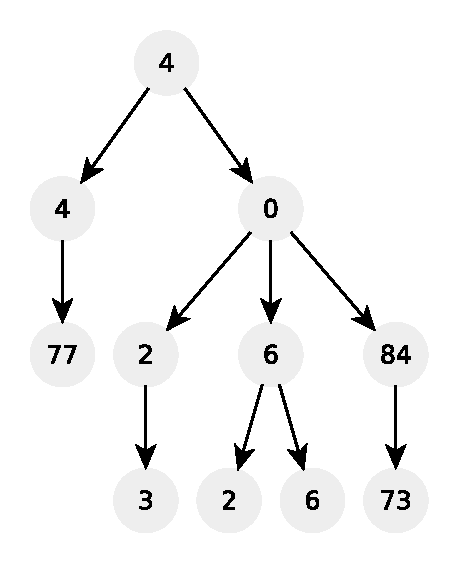
\includegraphics[width=1\linewidth]{sources/verify_BST/images/generic_tree}
		\caption[]{Example of a generic tree.}
		\label{fig:verify:generic_tree}
	 \end{subfigure}
	\hfill
	\begin{subfigure}[t]{0.46\textwidth}
		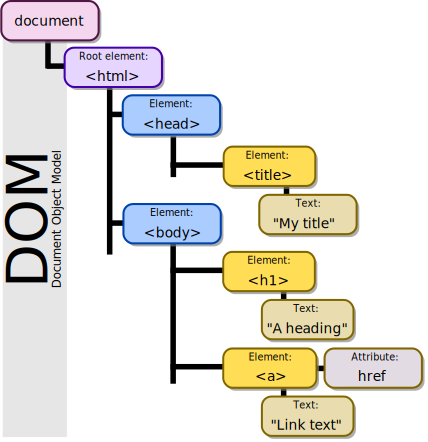
\includegraphics[width=1\linewidth]{sources/verify_BST/images/DOM-model}
		\caption[]{Example of DOM in a HTML document.}
		\label{fig:verify:DOM}
	 \end{subfigure}
	 \caption[]{}
	  \label{fig:verify:trees}
\end{figure}



Binary search trees (BST) are a special kind of trees that are extremely useful when we need to arrange data on which the following operations need to be performed
\begin{itemize}
	\item insert
	\item delete
	\item search
	\item ceil/floor
\end{itemize}.
In this chapter we are going to look at a common interview question in which we will have to determine whether a given tree is a valid BST or not. 
Studying this classic problem is important as the structure of and the insights behind it solutions can be transfered to many others trees problems.

\section{Problem statement}
\begin{exercise}
Given a binary tree \cite{cit:wiki:BST}, determine if it is a valid binary search tree (BST).

A BST is defined as follows:
\begin{itemize}
    \item the left subtree of a node contains only nodes with keys less than the node's key;
    \item the right subtree of a node contains only nodes with keys greater than the node's key.
\end{itemize}
You can assume the input tree is given as a pointer or a reference to a structure named \inline{TreeNode} which definition is in Listing \ref{list:verify_BST:tree_structure}. 

\end{exercise}

\begin{lstlisting}[language=c++, caption=Binary tree definition used in this exercice.,label=list:verify_BST:tree_structure]

 struct TreeNode {
     int val;
     TreeNode *left;
     TreeNode *right;
     TreeNode(int x) : val(x), left(nullptr), right(nullptr) {}
 };
 \end{lstlisting}


\begin{example}
	\label{example:verify_BST:example1}
	\hfill \\
	For the tree shown in Figure \ref{fig:verify:example1} the function should return \textbf{false}.
	
\end{example}

\begin{example}
	\label{example:verify_BST:example3}
	\hfill \\
	For the tree shown in Figure \ref{fig:verify:example3} the function should return \textbf{true}.
	
\end{example}

\begin{example}
\label{example:verify_BST:example4}
	\hfill \\
	For the tree shown in Figure \ref{fig:verify:example4} the function should return \textbf{true}.

\end{example}


\begin{figure}
	\vspace*{-0.5in}
	\centering
	\begin{subfigure}[t]{0.30\textwidth}
		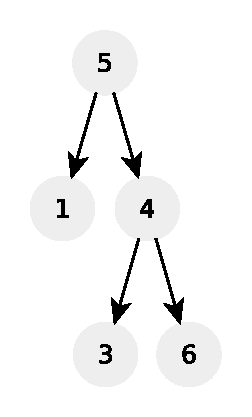
\includegraphics[width=1\linewidth]{sources/verify_BST/images/example1}
		\subcaption[]{Tree in Example \ref{example:verify_BST:example1}}
		\label{fig:verify:example1}
	 \end{subfigure}
	\hfill
	\begin{subfigure}[t]{0.30\textwidth}
		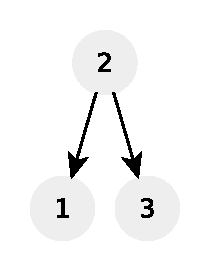
\includegraphics[width=1\linewidth]{sources/verify_BST/images/example3}
		\subcaption[]{Tree in Example \ref{example:verify_BST:example3}}
		\label{fig:verify:example3}
	 \end{subfigure}
	 \hfill
	 \begin{subfigure}[t]{0.30\textwidth}
		 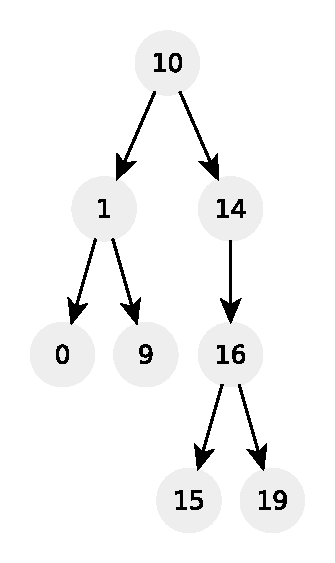
\includegraphics[width=1\linewidth]{sources/verify_BST/images/example4}
		 \subcaption[]{Tree in Example \ref{example:verify_BST:example4}}
		 \label{fig:verify:example4}
	  \end{subfigure}
	 \caption[]{}
	  \label{fig:verify:trees}
\end{figure}



\section{Clarification Questions}

\begin{QandA}
	\item \begin{questionitem} \begin{question} Is it guaranteed the input pointer or reference is valid tree?  \end{question} 	 
    \begin{answered}
		\textit{Yes, the input is a valid tree. There is a root, and all the other nodes have exactly one father.}
	\end{answered} \end{questionitem}
	\item \begin{questionitem} \begin{question} Are all elements in the tree distinct?  \end{question} 	 
    \begin{answered}
		\textit{Yes, you can assume all elemets are distinct.}
	\end{answered} \end{questionitem}
	\item \begin{questionitem} \begin{question} How many nodes does the tree contain?  \end{question} 	 
    \begin{answered}
		\textit{Up to $10^6$ nodes.}
	\end{answered} \end{questionitem}
\end{QandA}

\section{Discussion}
\label{verify_BST:sec:discussion}
In order to solve this problem, we need to write a function that is able to verify whether a given tree is a valid BST or not. But what does it mean to be valid exactly?
From the definition given above we know that tree $T$ is a BST when:
\begin{enumerate}
	\item Every node in $T$ has two subtree (which might be also empty and are named \textit{left} and \textit{right}, respectively). In other words, $T$ is a binary tree.
	\item given a node $n$ in the tree then \textbf{all} the nodes in its left subtree must be smaller than $n$;
	\item symmetrically, it must also hold that \textbf{all} nodes in the right subtree are larger than $n$.
\end{enumerate}
For instance, the tree in Figure \ref{ex:verify_BST:no_BST} is not a valid BST because node $15$ is a right descendant of the root but is it not greater than it. On the other hand, the trees in Figure \ref{example:verify_BST:example3} and \ref{example:verify_BST:example4} are valid BST. The tree in Figure \ref{fig:verify:generic_tree} is not a valid BST because it is not a binary tree as node $0$ has three children.

Therefore, in order to solve this problem we must be able to prove the conditions above hold for each and every node of the input tree. 

\subsection{A common mistake}
Most candidates can recall write down the BST properties rather quickly and they dive immediately into writing a greedy algorithm that works as follows: for each node $n$ of $T$ check that 
\inline{n.val > n->left.val && n.val < n->right.val} i.e. that the payload of the node currently  analyzed is greater than the value of its left child but smaller than its right one.
This algorithm might even return the correct answer for some input trees but it fails on others, and it is, therefore, not correct.
For example, it returns true if we execute on the tree in Figure \ref{ex:verify_BST:no_BST}.
Usually approching the problem this way means the end of the round and very likely  rejection. 

It becomes clear at this point, that the problem with this approach is that when verifying if the BST property holds for node $n$ we only look $n$ and its children. We must being able to check every node in the left and right subtrees of $n$ and also to somehow, make sure the information in $n$ travels down to $n$'s children and descendants so they can use it (to carry on the check for $n$ itself).
We will see how this can be done in the next sections.

\subsection{Top Down approach}
\label{verify_BST:sec:topdown}
When talking about trees, we should naturally be steered onto thinking about a top-down approach and recursion. 
In particular, this problem becomes almost trivial if approached using recursion and we are able to come up with the following insights:
\begin{enumerate}
	\item every node can be thought of as the root of a tree for which the BST property needs to be verified;
	\item empty trees satisfy the BST property by definition;
	\item every node must contain a value within a range that is determined by its ancestors. For instance, consider the node $15$ in the Figure \ref{example:verify_BST:example4}; it must be within the range $(14,16)$ for the tree to be a valid BST. Why is that? Because its parent, the node $16$ must be within the range $(14,+\infty)$ and additionally node $15$, being the left subtree of node $16$ must be lower than its parent. 
	The same reasoning can be applied recursively up to the root of the tree where the range of the value is simply $(-\infty, +\infty)$ (no constraints at all). 

	The node $9$ in the Figure \ref{example:verify_BST:example4} must be within the range $(1,10)$ for equivalent reasons.
\end{enumerate}

To summarize, we can visit the tree in a top-down fashion and maintain a range of values that the current node must satisfy. We can start with a range equal to $(-\infty, +\infty)$ for the root (meaning that de-facto, there is no restriction on the value the root can take).
Once the value is checked against this range, then the same function can be applied recursively to the right and left children but with the shrewdness of making sure that the range is modified accordingly when recurring on the children. 

The fulcrum of the problem seems to be the update of such a range change when visiting down the tree. How should it change when visiting a new node? 
The idea is quite simple:
Given a node $n$ with parent $p$ and range \( (l_p, u_p) \) then:
\begin{itemize}
	\item if $n$ is the right child of $p$, the range for $n$ is: $(p, u_p)$:
	all nodes in the right subtree of $p$ must be have a value \textbf{higher} than $p$. 
	Note that $p > l_p$ (otherwise the BST property would be violated when checking $p$) and thus the range for $n$ becomes smaller meaning that all the constraints coming from the ancestors of $p$ will also be satisfied with the new range $(p, u_p)$.
	\item A similar reasoning applies if $n$ is the left child of $p$: in this case, the range is $(l_u,p)$.
\end{itemize}
See Figure \ref{ex:verify_BST:example4_ranges} showing what the ranges look like for the tree in Figure \ref{ex:verify_BST:example4}. 


\begin{figure}
	\vspace*{-0.5in}
	\centering
	\begin{subfigure}[t]{0.52\textwidth}
		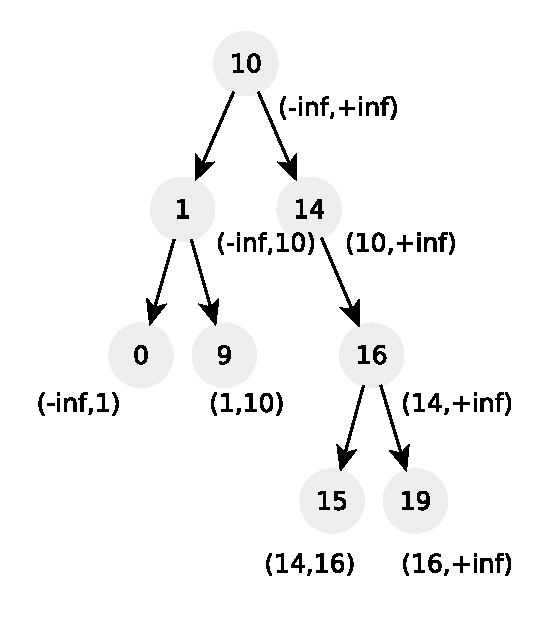
\includegraphics[width=1\linewidth]{sources/verify_BST/images/example4_ranges}
		\caption{Example of tree where each node is label with the range of values it should lie within.}
		\label{ex:verify_BST:example4_ranges}
	 \end{subfigure}
	\hfill
	\begin{subfigure}[t]{0.35\textwidth}
		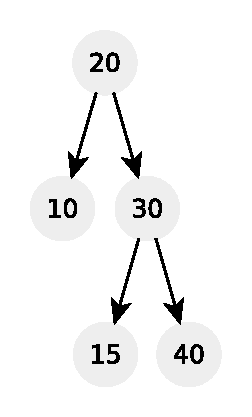
\includegraphics[width=1\linewidth]{sources/verify_BST/images/no_BST}
		\caption{Example of a binary tree that is not a BST.}
		\label{ex:verify_BST:no_BST}
	 \end{subfigure}
	 \caption[]{}
	  \label{fig:verify:trees_ranges_generic}
\end{figure}




An implementation of the idea above is shown in Listing \ref{list:verify_BST}. 

\lstinputlisting[language=c++, caption=Linear time recursive solution.,label=list:verify_BST]{sources/verify_BST/verify_BST_solution1.cpp}

The function \inline{isValidBST_top_down} is a simple entry point for the recursive function \inline{isValidBST_top_down_helper} which uses the parameters \inline{lower} and \inline{upper} to keep track of the range the node \inline{root} must respect. 
The interesting bits in this function are the ways the recursive calls are made and specifically in what values are provided to the parameters \inline{lower} and \inline{upper}. 
When performing the first recursive call on \inline{root->left} the parameter \inline{lower} is kept unchanged while the \inline{upper} is set to be equal to the current value of root because every element in the left subtree of $n$ must indeed be smaller than \inline{root->val}.

Symmetrically for the second recursive call on \inline{root->right}, \inline{upper} stays unchanged and \inline{lower} get the value of \inline{root->val} because all the nodes in $n$'s right subtree must be larger than \inline{root->val}.

The time and space complexities of Listing \ref{list:verify_BST} are $O(n)$  and $O(1)$, respectively space (if we do not keep into consideration the space on the stack taken by the recursion).

\subsection{Brute force}
We can look at the problem from a different perspective and try to prove the input tree is not  BST rather than trying to prove it is. Clearly, if we fail as proving it is not a BST, then it must indeed be one!
A tree is not a BST if we are able to find a node $n$ s.t. its left subtree contains any element greater than $n$ and or its right subtree contains any element smaller than $n$.
This task is trivial when the two following functions are available:
\begin{enumerate}
	\item \inline{tree_min(TreeNode* root)}
	\item \inline{tree_max(TreeNode* root)}
\end{enumerate}.
which return the minimum and the maximum value of a tree, respectively.

We can verify the BST property of a node $n$ is not violated by making sure that the maximum value in its left subtree is not larger or equal than $n$ and that the minimum value in its right subtree is not smaller or equal than $n$.

Luckly implementing \inline{tree_min(TreeNode* root)} and \inline{tree_max(TreeNode* root)} is easy to do in linear time as all we need to do is traverse the tree (in any order really) and keep track of the smallest/largest element seen. 

The idea above can be implemented as shown in Listing \ref{list:verify_BST_bruteforce}

\lstinputlisting[language=c++, caption=Quadratic solution based on the two functions returning the minimum and maximum value of a tree.,label=list:verify_BST_bruteforce]{sources/verify_BST/verify_BST_solution2.cpp}

Listing \ref{list:verify_BST_bruteforce} has a quadratic time complexity because for each and every node of the tree we perform a linear amount of work. The space complexity is also linear if we consider the space on the stack to perform the recursion.


Notice that we can do substantially better than quadratic time if we memoize \inline{tree_min} and \inline{tree_max} at the expense of using linear space. We can, for instance, use a map to store the information for each \inline{TreeNode*} and its associated min and max values. An implementation of this idea is shown in Listing \ref{list:verify_BST_bruteforce_improved}.

\lstinputlisting[language=c++, caption=Linear time solution obtained by memoizing Listing \ref{list:verify_BST_bruteforce_improved}.,label=list:verify_BST_bruteforce]{sources/verify_BST/verify_BST_solution3.cpp}
